\documentclass[11pt]{article}

\usepackage[a4paper,
            bindingoffset=0.5cm,
            left=3cm,
            right=3cm,
            top=3cm,
            bottom=4cm,
            footskip=1.5cm]{geometry}
            
%
\usepackage[T1]{fontenc}
\usepackage{graphicx}
\usepackage{enumitem}
\usepackage{blindtext}
\usepackage{float}
\usepackage{xcolor}
\usepackage{multirow}
\usepackage{minted}
 \usepackage{url}
%

\setcounter{secnumdepth}{3}

%%%%%%%%%%%%%%%%%%%%%
\title{\textbf{Critical Systems Lab - MESCC\\ Water Pumping Automated System}}
\date{ISEP, January 2024, \textbf{Second Delivery}}
\author{Ricardo Mendes\\ 1201779
\and Arthur Gerbelli\\ 1220201}
%%%%%%%%%%%%%%%%%%%%%

\begin{document}

\maketitle              
\newpage
\tableofcontents
\newpage

%
\section{Introduction}

This document is a follow-up of the previous work.

It takes into account the feedback received during the last presentation and also the current objectives of the exercise.

%%%
\section{Requirement Specification}

%%%
\subsection{Problem Domain}

%%%
\subsubsection{[UPDATED] Stakeholder Needs}

Although not mentioned on the assignment, we chose to add some changes to the Stakeholder Needs that are paramount to understand the next chapters.

\begin{itemize}
	\item \textbf{SN-1.3} Every WPS will have two pumps and two water level sensors to achieve a certain level of redundancy and reliability on the system.
	\item \textbf{SN-1.4} To improve the system's performance, and given that we have one unused water pump, this pump should be used when the water level is above 2/3 of the well max capacity.
	\item \textbf{SN-1.5} In case that only one water pump is operational, the max capacity of the WPS shall be reduced.
\end{itemize}

\textbf{SN-1.4} and \textbf{SN-1.5} are the result of the Stakeholder being able to describe the system's performance using the identified \textit{Measure of Effectiveness}. The wet well capacity and the input flow can be greater if we use the second pump instead of leaving it on stand-by and only used during failure.

As described in the Stakeholder Needs, the second pump will work only if the water level is above 2/3 of the well capacity. In case that one of the pumps stops to be operational, an alarm will be triggered to alert the maintenance team, and the max. water level will be reduced.

\subsubsection{[UPDATED] System Context and Use Cases}

During the previous analysis of the System's Context and Use Cases, we decided to split the WPS system as a whole. The main objective is to split responsibilities and so, simplifying and clarifying the requirements. Another result, was the creation of two, very easy to grasp, systems: the RSS and the WPS. 

By turning it simple, we can state that the system has obviously no bugs; on a complex one, we can only which to achieve a system with no obvious bugs.

The following changes were made in the Use Case diagrams:

\begin{figure}[H]
\centering
\begin{minipage}{.5\linewidth}
  \centering
  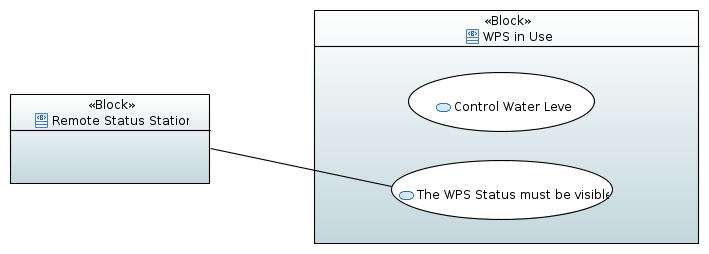
\includegraphics[width=150px]{../diagrams/use-case-wps.png}
  \caption{Use Case diagram - WPS}
  \label{fig:Use Case WPS}
\end{minipage}%
\begin{minipage}{.5\linewidth}
  \centering
  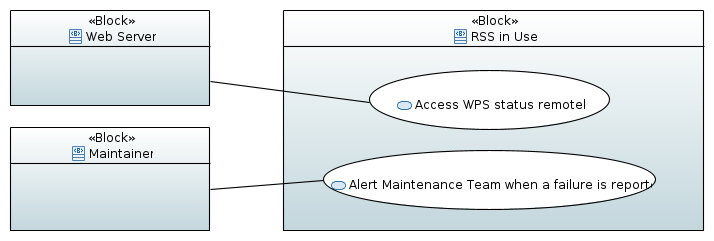
\includegraphics[width=150px]{../diagrams/use-case-rss.png}
  \caption{Use Case diagram - RSS}
  \label{fig:Use Case RSS}
\end{minipage}
\end{figure}

The activity diagram of the use case \textit{"Control Water Level"}, also shows that WPS can be seen as an independent system regarding the RSS.

The interactions are between the sensors, the water pump as the main actuator, and the control unit.

So one of the externalities of the WPS, is to give visibility to its internal status.

\begin{figure}[H]
  \centering
  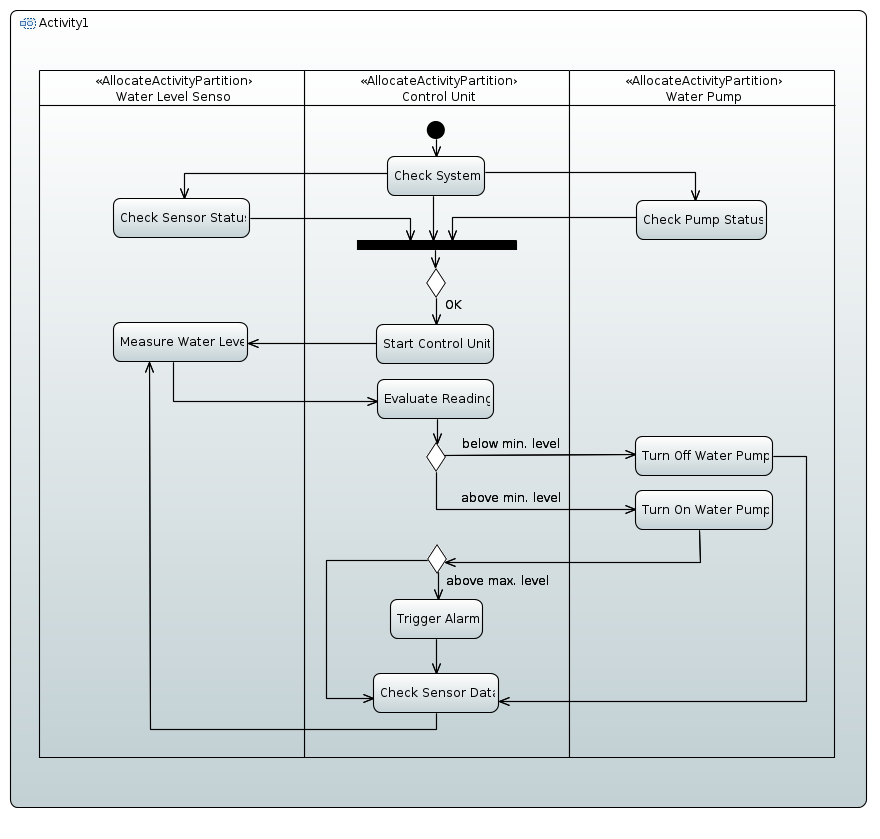
\includegraphics[width=300px]{../diagrams/use-case-activity-diagram-01.png}
  \caption{Control the Water Level inside the well}
  \label{fig:Control Water Level Activity Diagram}
\end{figure}

%%%
\subsection{Solution Domain}

%%%
\subsubsection{Hazard Analysis}

Given the critical nature of the system, we reintroduced here an updated analysis of its hazards. This list maps directly to the Stakeholder Need SN-1.3 but goes a little bit further.

\begin{enumerate}[leftmargin=4em, font=\small, label=\textbf{H-\arabic*:}]
	\setlength\itemsep{.5em}
	\item 
		\begin{itemize}
		\setlength\itemsep{0em}
        	\item \textbf{Description:} One of the pumps stops working.
			\item Cause: Mechanical problem.
    		\item Effect: Lost of redundancy and reduction of system performance.
    		\item \textbf{Mitigation:} Reduce the maximum water level to 2/3 and trigger alarm.
		\end{itemize}
	\item 
		\begin{itemize}
		\setlength\itemsep{0em}
    		\item \textbf{Description:} Both pumps stopped working.
			\item Cause: Mechanical problem.
    		\item Effect: Complete failure of the system.
    		\item \textbf{Mitigation:} Trigger alarm.
		\end{itemize} 	
	\item 
		\begin{itemize}
		\setlength\itemsep{0em}
    		\item \textbf{Description:} A pump doesn't turn OFF when the water level in bellow minimum.
			\item Cause: Mechanical problem.
    		\item Effect: Pump overheating and complete failure.
    		\item \textbf{Mitigation:} Trigger alarm.
		\end{itemize} 
	\item 
		\begin{itemize}
		\setlength\itemsep{0em}
    		\item \textbf{Description:} The two level sensors give contradictory readings, i.e. one above max and one below min.
			\item Cause: Sensor malfunction, connection issues.
    		\item Effect: Inappropriate system behavior. 
    		\item \textbf{Mitigation:} If the reading of both sensor are too unequal, there must be a way to distinguish between the wrong and the correct data. There are three possible ways to deal with the issues: choose a master and a slave sensor, retain the previous input and compare it with the current one, or choose the worst case. Trigger the alarm if the system in unable to achieve a consensus.
		\end{itemize}
	\item 
		\begin{itemize}
		\setlength\itemsep{0em}
    		\item \textbf{Description:} Power shortage.
			\item Cause: Multiple causes
    		\item Effect: Complete failure of the system.
    		\item \textbf{Mitigation:} RSS with independente power supply and trigger alarm.
		\end{itemize} 
	\item 
		\begin{itemize}
		\setlength\itemsep{0em}
    		\item \textbf{Description:} RSS are not getting information from WPS.
			\item Cause: Connection issues or Messagem broker stoped working.
    		\item Effect: Unknown status of the system.
    		\item \textbf{Mitigation:} Implement a cluter of MQTT Brokers or remove this single point of failure by adopting DDS.
		\end{itemize} 
	\item 
		\begin{itemize}
		\setlength\itemsep{0em}
    		\item \textbf{Description:} RSS stops working.
			\item Cause: Malfunction.
    		\item Effect: Unknown WPS status.
    		\item \textbf{Mitigation:} Have redundancy by having multiple RSS and each one displaying all statuses from all WPS.
		\end{itemize} 
	\item 
		\begin{itemize}
		\setlength\itemsep{0em}
    		\item \textbf{Description:} Control Unit stops working.
			\item Cause: Malfunction, bug.
    		\item Effect: Total failure of the system.
    		\item \textbf{Mitigation:} Implement redundancy by having a cluster of nodes running the Control Unit. If the number of nodes is 3 we can implement a voting system and run the same process with the same input in parallel. This would improve the system's fault tolerance.
		\end{itemize} 
\end{enumerate}


The main output of this analysis was an updated System Requirements.


%%%
\subsubsection{[UPDATED] System Requirements}

\begin{enumerate}[leftmargin=4em, font=\small, label=\textbf{SR-\arabic*}]
	\setlength\itemsep{.5em}
	\item 

		\begin{enumerate}[leftmargin=1.5em, font=\small, label=\textbf{.\arabic*:}]
		\setlength\itemsep{0em}
		\item \textcolor{gray}{While the water level is above the minimum level, WPS shall have a pump working.}
		\item \textcolor{gray}{When the water level is below minimum level, WPS shall have all pumps stopped.}
		\item \textcolor{gray}{If the water level is above the maximum level, then the WPS shall trigger an alarm at the Remote Status Station (RSS).}
		
		\item A second pump shall be turned on only when the water level is above 2/3 the maximum water level.
		\item When only one pump is available, the maximum water level shall be reduced to 2/3.
		\item If the readings of the sensor are uneven to a level of 20cm, the system should choose the worst case scenario, following the table below: 
		
\begin{table}[H]
\begin{tabular}{lrllll}
                                               & \multicolumn{1}{l}{}            & \multicolumn{4}{l}{sensor \#1}                                                                                                          \\ \cline{3-6} 
                                               & \multicolumn{1}{l|}{}           & \multicolumn{1}{l|}{\textbf{0}} & \multicolumn{1}{l|}{\textbf{1}} & \multicolumn{1}{l|}{\textbf{2}} & \multicolumn{1}{l|}{\textbf{3}} \\ \cline{2-6} 
\multicolumn{1}{l|}{\multirow{4}{*}{sensor \#2}} & \multicolumn{1}{r|}{\textbf{0}} & \multicolumn{1}{l|}{0}          & \multicolumn{1}{l|}{0}          & \multicolumn{1}{l|}{0}          & \multicolumn{1}{l|}{3}          \\ \cline{2-6} 
\multicolumn{1}{l|}{}                          & \multicolumn{1}{r|}{\textbf{1}} & \multicolumn{1}{l|}{0}          & \multicolumn{1}{l|}{1}          & \multicolumn{1}{l|}{1}          & \multicolumn{1}{l|}{3}          \\ \cline{2-6} 
\multicolumn{1}{l|}{}                          & \multicolumn{1}{r|}{\textbf{2}} & \multicolumn{1}{l|}{0}          & \multicolumn{1}{l|}{1}          & \multicolumn{1}{l|}{2}          & \multicolumn{1}{l|}{3}          \\ \cline{2-6} 
\multicolumn{1}{l|}{}                          & \multicolumn{1}{r|}{\textbf{3}} & \multicolumn{1}{l|}{3}          & \multicolumn{1}{l|}{3}          & \multicolumn{1}{l|}{3}          & \multicolumn{1}{l|}{3}          \\ \cline{2-6} 
\end{tabular}
\end{table}

\textbf{0} = below min; \textbf{1} = above min; \textbf{2} = above med; \textbf{3} = above max.
		\end{enumerate}
		
	\item
		\begin{enumerate}[leftmargin=1.5em, font=\small, label=\textbf{.\arabic*:}]
		\setlength\itemsep{0em}
		\item \textcolor{gray}{The status of all WPS shall be displayed on all RSS.}
		\item \textcolor{gray}{If the alarm is ON, the button in the RSS shall only disable it.}
		\item The RSS shall have an independent power supply from the WPS.
		\item The alarm on the RSS shall have an independent power supply from the RSS itself and from the WPS.
		\end{enumerate}
	
	\item	
		\begin{enumerate}[leftmargin=1.5em, font=\small, label=\textbf{.\arabic*:}]
		\setlength\itemsep{0em}
		\item \textcolor{gray}{The status of all WPS shall be visible on a web page.}
		\end{enumerate}

	\item
		\begin{enumerate}[leftmargin=1.5em, font=\small, label=\textbf{.\arabic*:}]
		\setlength\itemsep{0em}
		\item To improve the system´s communication reliability, a cluster of 2(two) MQTT brokers shall be deployed.
		\end{enumerate}

\end{enumerate}

%%%
\subsubsection{[UPDATED] System Structure}

As already stated during the System's Context analysis, we chose to split the system into two main system. This is mainly based on the principle of single responsibility.

The result can be seen below:

\begin{figure}[H]
  \centering
  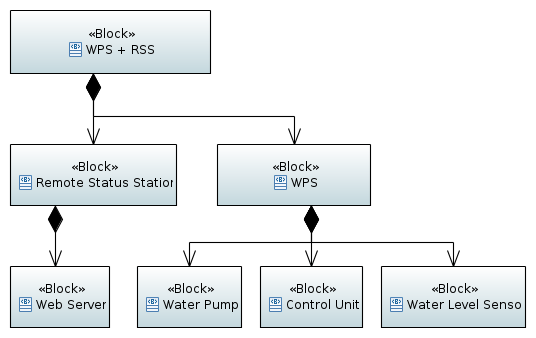
\includegraphics[width=300px]{../diagrams/system-structure.png}
  \caption{System Structure Diagram}
  \label{fig:System Structure Diagram}
\end{figure}

%%%
\subsubsection{Traceability}

This chapter should clarify that the results from the Problem Domain and the analysis of the Solution Domain map to the final system implementation.

The Stakeholder Needs are being answered by the Requirements that we documented:

\begin{figure}[H]
  \centering
  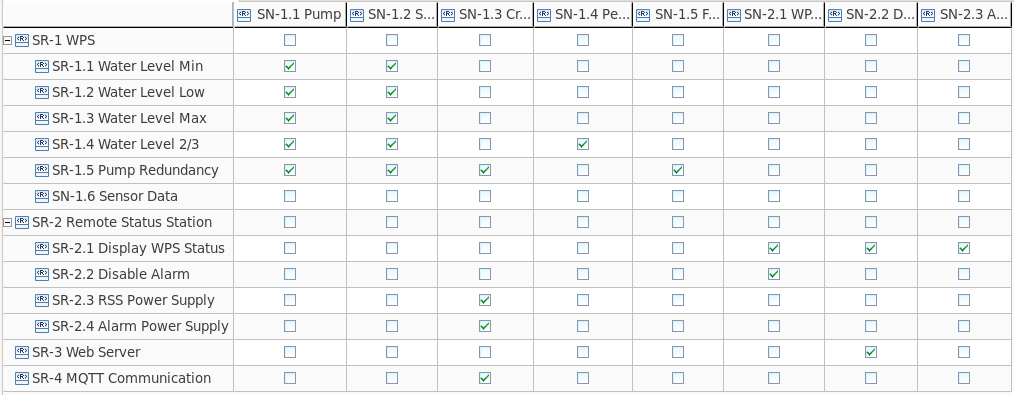
\includegraphics[width=\linewidth]{../diagrams/traceability.png}
  \caption{Traceability to Stakeholder Needs}
  \label{fig:Traceability}
\end{figure}

The diagram, developed during the analysis of the System Structure, is being used as the main foundation of the deployment diagram (please see the diagram on the \textit{Implementation} chapter.

Most important, the Hazard analysis gave raise to multiple new requirements, that although not obvious in the Stakeholder Needs, are here handled critical for the description of the system.

\newpage
%%%
\section{Implementation}

%%%
\subsection{Concorrency and Real Time Scheduling}

%%%%
\subsubsection{Introduction}

To give a realistic analysis of the processes that we are here proposing to run, we need first to describe the hardware where they will be running.

The microcontroller ESP32 has FreeRTOS integrated into as a component, however in our case some there is a sligh difference:
\newline
\newline
 \textit{The original FreeRTOS (...) is a compact and efficient real-time operating system supported on numerous single-core MCUs and SoCs. However, to support dual-core ESP targets, such as ESP32, ESP32-S3, and ESP32-P4, ESP-IDF provides a unique implementation of FreeRTOS with dual-core symmetric multiprocessing (SMP) capabilities (hereinafter referred to as IDF FreeRTOS).}\cite{c1}
\newline
\newline
So we are dealing with a textbf{fixed priority preemptive scheduler with time slicing}, meaning:

\begin{itemize}
	\item Each task is given a constant priority upon creation.
	\item The scheduler can switch execution to another task without the cooperation of the currently running task.
	\item The scheduler periodically switches execution between ready-state tasks of the same priority in a round-robin fashion. 
\end{itemize}

%%%%
\subsubsection{Concorrency}

\subsubsection{Real Time Scheduling}

%%%
\newpage
\subsection{Communication Infrastructure}

The following text describes the prototype that we propose to implement. 

\begin{figure}[H]
  \centering
  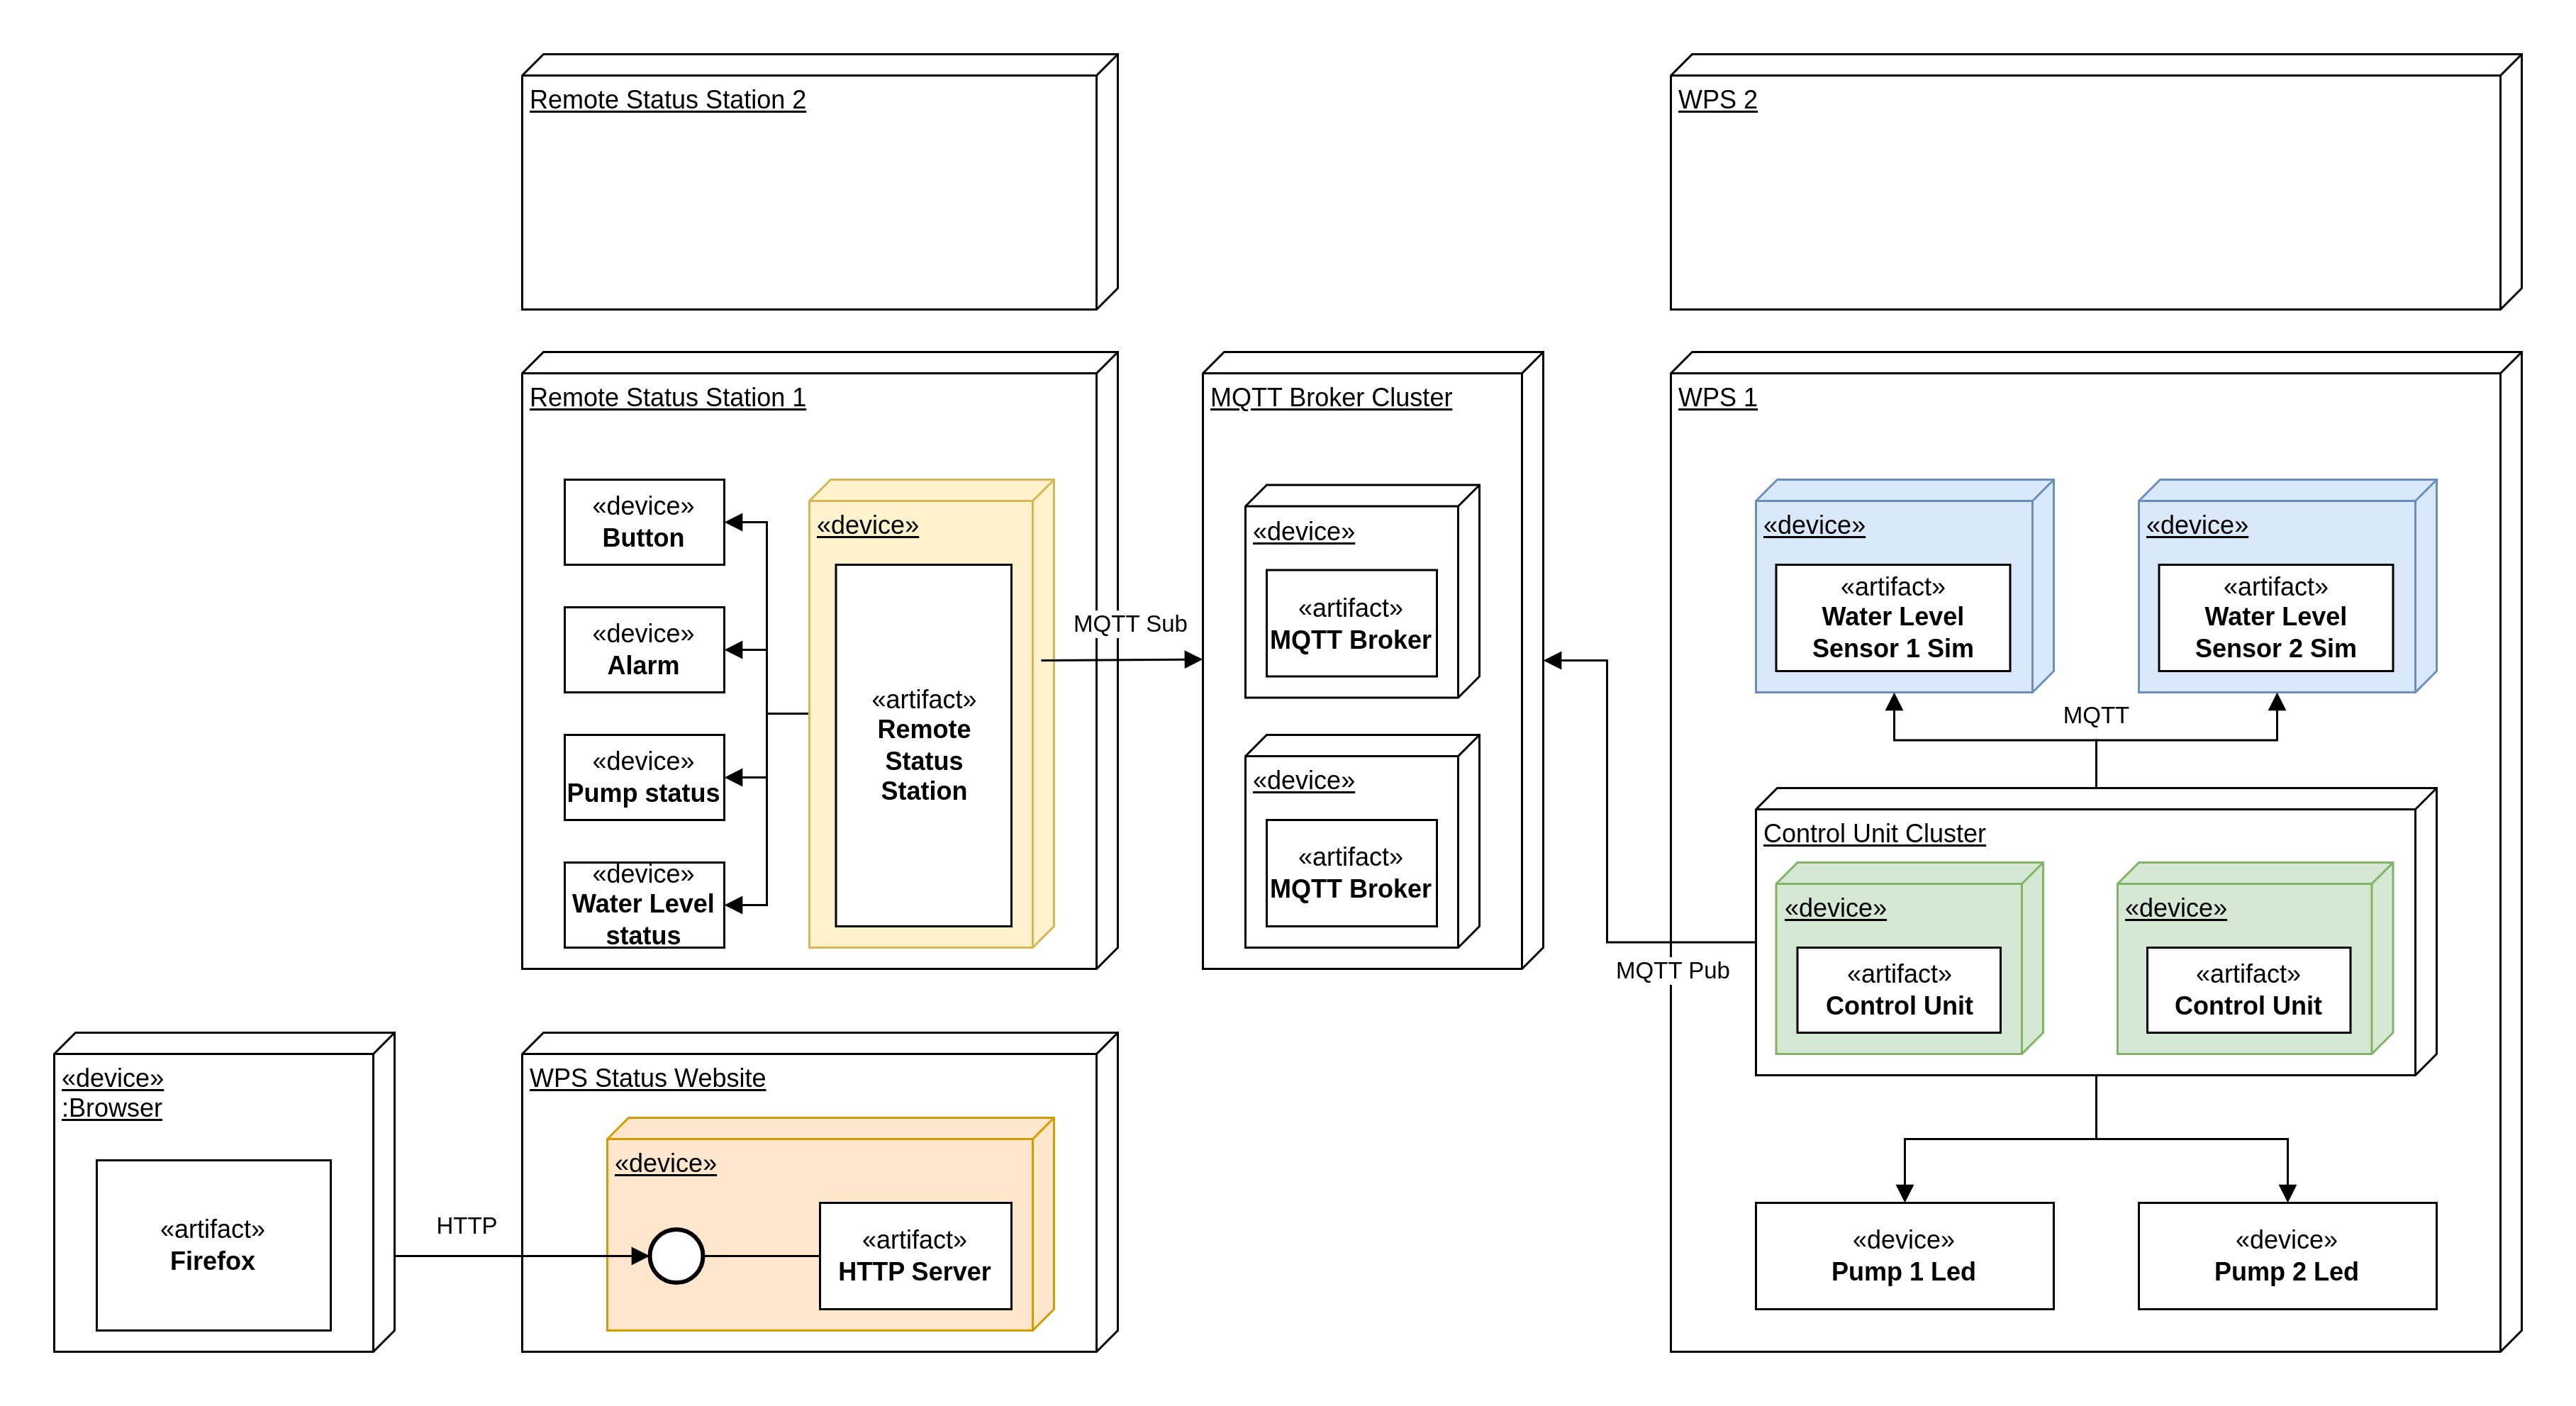
\includegraphics[width=\linewidth]{../diagrams/deployment-diagram-WPS.jpg}
  \caption{Deployment diagram}
  \label{fig:Deployment Diagram}
\end{figure}

\textbf{Communication Software Infrastructure:}

\begin{itemize}
	\item The Web Server will be implemented using the Apache HTTP Server and will run on a Raspberry Pi 4.
	\item The MQTT Brokers will be implemented using Mosquitto MQTT and will run on a Raspberry Pi 4.
	\item The Sensors and Control Unit will run on Arduinos ESP32 and will be implemented using 'C' with the help of some Arduino Libraries. 
\end{itemize}

\textbf{Interactions between elements:}

The main communication protocol is MQTT. The only publisher is the Control Unit in the WPS. The Web Server and the RSS are the subscribers.

The communication made between Control Unit and Water Sensor will be TCP/IP through wireless. Given that it is a critical system, the Control Unit will query the sensor in regular intervals and asking for the data.

A time-out or incorrect data sent by the sensor can trigger an alert to the RSS. Essencially is a pull strategy from the point of view of the critical system.

The Web Client will interact with the HTTP Server using the HTTP protocol.

All other connection shown in the diagram area physical connection inside a bread-board.

%%%
\newpage
\subsection{Assembly}

The piece of functionality that we choosed to write in assembly is located in the sensor simulator.

The sensor simulator has four push buttons. Each button triggers a different change in the water level. 
The current water level can be seen by the LED that is turned on.

\begin{figure}[H]
  \centering
  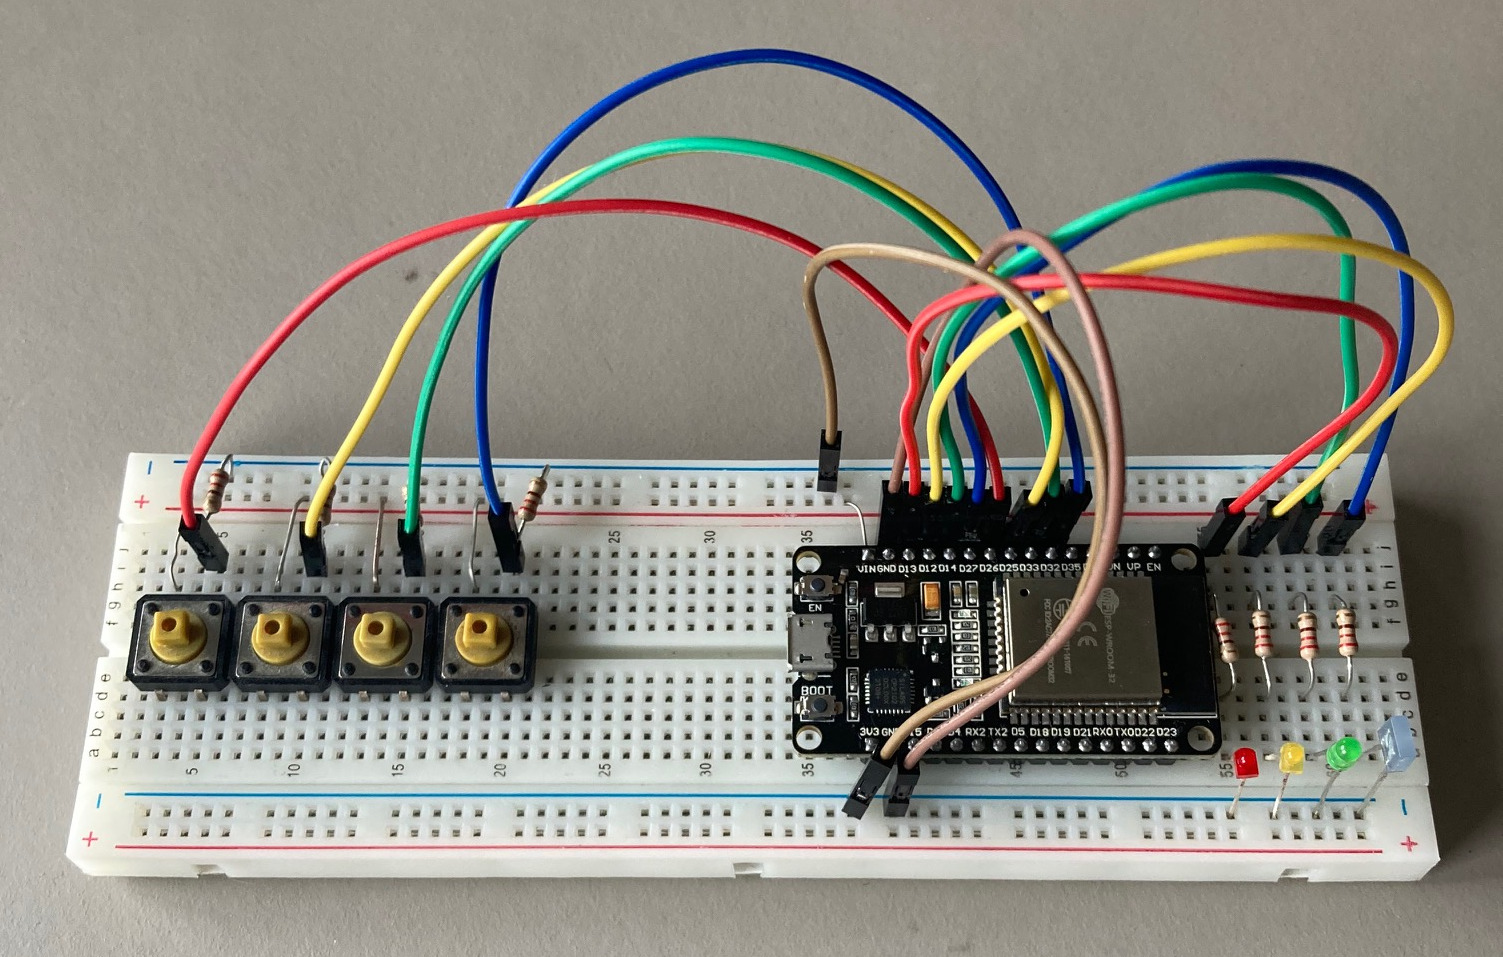
\includegraphics[width=300px]{../diagrams/sensor-sim-01.jpg}
  \caption{Sensor Sim prototype}
  \label{fig:Sensor sim prototype}
\end{figure}

Because only one water level state is possible we choose to use assembly to create a mask to be implemented on the leds.

\begin{minted}{gas}
.global getMask

getMask:    entry a1, 48
            movi a5, 0          # init increment
            mov a6, a2          # save inputed water level
            movi a2, 1          # init return value

loop: 
            addi a5, a5, 1      # increment by one
            beq a5, a6, end     # branch to 'end' if not equal
            slli a2, a2, 1      # left shif by 1, i.e. 0001 -> 0010
            j loop              # jump to loop 

end:
            retw.n
\end{minted}

For example, if we push the BUTTON\_MIN (the green one), this will trigger the code above and output the following number \textbf{2} that corresponds to \textbf{0000 0010} in a 1 byte binary. 

The code below, then implements the mask:

\begin{minted}{c}
void implementMask(int8_t mask)
{
  int8_t n_bit = 0;
  while (n_bit < MAX_LEVELS) {
    if (mask & 0x01) {
      digitalWrite(STATES[n_bit], HIGH);
    }
    else {
      digitalWrite(STATES[n_bit], LOW);
    }
    n_bit++;
    mask = mask >> 1;
  }
}
\end{minted}

%%%%%%%%%%%%%%%%%%%%%
\newpage
\begin{thebibliography}{8}

\bibitem{c1}
 Espressif documentation: {\url{https://docs.espressif.com/projects/esp-idf/en/latest/esp32/api-reference/system/freertos_idf.html#id23/}}

\end{thebibliography}

\end{document}
